\section{Informal development}
\label{sec:intuition}

We illustrate all four new reasoning principles of \colosl by
sketching a proof of a simple, if slightly artificial, example.  We will look
at less contrived examples in \S\ref{sec:examples}. Consider the
program $\mathbb{INC}$ defined in Figure~\ref{.}, ignoring the
assertions. It is written in pseudo-code, where variables $x$, $y$ and
$z$ are allocated on the heap and variable reading and mutation are
understood as the corresponding heap operations. After initialisation
of the variables to $0$, three threads are spawned to increment each
variable in a lock-step fashion: $\mathbb{P}_x$ is the first allowed
to run its increment operation; then $\mathbb{P}_y$; and finally
$\mathbb{P}_z$. This process repeats until $x = y = z = 10$.  This
example code is interesting because the threads are intrically
intertwinned. With thread $\mathbb{P}_y$, the programmer
knows that the resource directly affected by the thread involves the cells
given by $x$ and $y$. He knows the 
simple  behaviour of the thread that 
 it will increment the cell at $y$ as long as it is less than $x$.
However, he also knows a
much more complex  behaviour associated with the resource of  the thread that,  given the initial
 condition that all the cells have value $0$, then the thread can only
 increase  $y$ by $1$ if 
$x$ is  one more than $y$  and the environment can only  increase
$x$ by one if 
$x$ and $z$ (and in fact  $y$) have the same value. Finally, the
programmer knows that the end result will be that the value of the
cells given by $x$, $y$ and $z$ will be $10$. 



\pgcomment{I need line numbers on INC and Py to describe
  properly. need [x] all over the place.} 


\begin{figure*}
\centering
\begin{tabular}{@{}l@{\ }|@{\ }l@{\ }|@{\ }l@{\ }|@{\ }l@{}}
  {$\mathbb{P}_x$:}& 
  {$\mathbb{P}_y$:}& 
  {$\mathbb{P}_z$:}&
  $\mathbb{INC}$:\\[.5ex]
\begin{lstlisting}
//$\comment\{\shared{\cell{z}{0} * \cell{x}{0}}{I_x} * \token a_x\}$
while($x$ != 10)
//$\comment\left\{\shared{\begin{array}{@{}l<{\null}@{}l<{\null}@{}}\exsts{v}\cell{z}{v} * \cell{x}{v} \lor\\ \cell{z}{v} * \cell{x}{v+1}\end{array}}{I_x}\!\!\!\!\!\! * \token a_x\right\}$
{ $\langle$if ($x$ == $z$) $x$++;$\rangle$ }
//$\comment\left\{\shared{\begin{array}{@{}l<{\null}@{}l<{\null}@{}}\cell{z}{10} * \cell{x}{10} \lor\\ \cell{z}{9} * \cell{x}{10}\end{array}}{I_x}\!\!\!\!\!\! * \token a_x\right\}$
\end{lstlisting}
&
\begin{lstlisting}
//$\comment\left\{\shared{\begin{array}{@{}l<{\null}@{}l<{\null}@{}}\cell{x}{0} * \cell{y}{0} \lor\\ \cell{x}{1} * \cell{y}{0}\end{array}}{I_y}\!\!\!\!\!\! * \token a_y\right\}$
while($y$ != 10)
//$\comment\left\{\shared{\begin{array}{@{}l<{\null}@{}l<{\null}@{}}\exsts{v}\cell{x}{v} * \cell{y}{v} \lor\\ \cell{x}{v+1} * \cell{y}{v}\end{array}}{I_y}\!\!\!\!\!\! * \token a_y\right\}$
{ $\langle$if ($y$ < $x$) $y$++;$\rangle$ }
//$\comment\left\{\shared{\begin{array}{@{}l<{\null}@{}l<{\null}@{}}\cell{x}{10} * \cell{y}{10} \lor\\ \cell{x}{11} * \cell{y}{10}\end{array}}{I_y}\!\!\!\!\!\! * \token a_y\right\}$
\end{lstlisting}
&
\begin{lstlisting}
//$\comment\left\{\shared{\begin{array}{@{}l<{\null}@{}l<{\null}@{}}\cell{y}{0} * \cell{z}{0} \lor\\ \cell{y}{1} * \cell{z}{0}\end{array}}{I_z}\!\!\!\!\!\! * \token a_z\right\}$
while($y$ != 10)
//$\comment\left\{\shared{\begin{array}{@{}l<{\null}@{}l<{\null}@{}}\exsts{v}\cell{y}{v} * \cell{z}{v} \lor\\ \cell{y}{v+1} * \cell{z}{v}\end{array}}{I_z}\!\!\!\!\!\! * \token a_z\right\}$
{ $\langle$if ($z$ < $y$) $z$++;$\rangle$ }
//$\comment\left\{\shared{\begin{array}{@{}l<{\null}@{}l<{\null}@{}}\cell{y}{10} * \cell{z}{10} \lor\\ \cell{y}{11} * \cell{z}{10}\end{array}}{I_z}\!\!\!\!\!\! * \token a_z\right\}$
\end{lstlisting}
&
\begin{lstlisting}
//$\comment\{x|-> - * y|-> - * z|-> - \}$
$x$ = 0; $y$ = 0; $z$ = 0;
//$\comment\{x|-> 0 * y|-> 0 * z|-> 0 \}$
//$\comment\left\{\begin{array}{@{}l<{\null}@{}l<{\null}@{}}\shared{x|-> 0 * y|-> 0 * z|-> 0} I\\ \null*\token a_x * \token a_y * \token a_z\end{array}\right\}$
($\mathbb{P}_x$ || $\mathbb{P}_y$ || $\mathbb{P}_z$)
//$\comment\left\{\begin{array}{@{}l<{\null}@{}l<{\null}@{}}\shared{x|-> 10 * y|-> 10 * z|-> 10} I\\ \null*\token a_x * \token a_y * \token a_z\end{array}\right\}$
\end{lstlisting}
\end{tabular}

\begin{minipage}{.2\textwidth}
\begin{align*}
  I_x &\eqdef \left\{
  \begin{array}{@{}l@{}}
    \token a_x:\, \exsts{v} \cell{z}{v} * \cell{x}{v}  \swap  \cell{z}{v} * \cell{x}{v+1}\\
    \token a_z:\, \exsts{v} \cell{x}{v+1} * \cell{y}{v+1} * \cell{z}{v}\swap \cell{x}{v+1} * \cell{y}{v+1} * \cell{z}{v+1}
  \end{array}
  \right.\\
  I_y &\eqdef \left\{
  \begin{array}{@{}l@{}}
    \token a_x:\, \exsts{v} \cell{x}{v} * \cell{y}{v} * \cell{z}{v}  \swap  \cell{x}{v+1} * \cell{y}{v} * \cell{z}{v}\\
    \token a_y:\, \exsts{v} \cell{x}{v+1} *  \cell{y}{v}\swap \cell{x}{v+1} * \cell{y}{v+1}
  \end{array}
  \right.\\
  I_z &\eqdef \left\{
  \begin{array}{@{}l@{}}
    \token a_y:\, \exsts{v} \cell{x}{v+1} * \cell{y}{v} * \cell{z}{v}  \swap \cell{x}{v+1} * \cell{y}{v+1} * \cell{z}{v}\\
    \token a_z:\, \exsts{v} \cell{y}{v+1} *  \cell{z}{v}\swap \cell{y}{v+1} * \cell{z}{v+1}
  \end{array}
  \right.
\end{align*}
\end{minipage}\quad\ 
\begin{minipage}{.2\textwidth}
\begin{align*}
  I &\eqdef \left\{
  \begin{array}{@{}l@{\,}l@{}l@{}}
    \token a_x: & \exsts{v} & \cell{z}{v} * \cell{x}{v} \swap\\
    &&\quad \cell{z}{v} * \cell{x}{v+1}\\
    \token a_y: & \exsts{v} & \cell{x}{v+1} * \cell{y}{v} \swap \\
    &&\quad \cell{x}{v+1} * \cell{y}{v+1}\\
    \token a_z: & \exsts{v} & \cell{y}{v+1} * \cell{z}{v} \swap \\
    &&\quad \cell{y}{v+1} * \cell{z}{v+1}
  \end{array}\right.
\end{align*}
\end{minipage}

\vspace{5pt}\hrule\vspace{5pt}
\caption{The concurrent increment program together with a \colosl proof
  sketch. Lines starting with \lstinline{//} contain formulas that describe
  the local state and the subjective shared state at the relevant program point.}
\label{fig:concurrentInc}
\end{figure*}


\colosl
can quite simply specify this complex behaviour of the
resource associated with thread
$\mathbb{P}_y$. 
\colosl assertions comprise  standard assertions from the
separation-logic literature~\cite{rey02,sepish,variablesasresource},
plus {\em subjective views} and {\em capabilities}. \colosl
assertions are interpreted over a particular domain which includes:
{thread-local} state exclusively visible to the thread; {\em one}
global shared state accessible by all threads; and { interference
actions}  describing how the global state can be updated. An 
subjective view  $\shared{P} I$ comprises assertion $P$ which
gives {\em partial} information about the global
shared state and interference relation $I$  which gives partial
information about  how this
part of the shared state may change by declaring actions of the form  $\token a :
P' \swap Q$.  A capability assertion $[\token a]$ provides a thread with permission to 
change that partial shared state using action $\token a$.




Consider the \colosl assertions associated with $\mathbb{INC}$.
After
initialisation, line~?? of $\mathbb{INC}$  provides a standard
assertion from separation logic stating that 
the thread-local state consists of three  heap cells,  which are
referred to by  variables $x$,
$y$ and $z$ and contain the value  $0$. This resource in the thread-local state is
fully owned by  the thread. Using the extension principle, the thread is able to give up  this local
resource and transfer it  to the global shared state. For example, line~?? demonstates the
creation of a subjective view $\shared{x|-> 0 * y|-> 0 * z|->
  0}I$, where {part} of the underlying
global shared state now contains the three heap cells and the 
interference relation $I$ declares  how  this  part of the  shared state  is able 
change. For example,  the action 
\[
 \token a_y:  \exsts{v} \cell{x}{v+1} * \cell{y}{v} \swap 
    \quad \cell{x}{v+1} * \cell{y}{v+1}
\]
can increment  the cell given by $y$ under the condition that the
value of the  cell
given by $x$ is one more than that of $y$. 
This update is only possible when the
local state of a thread has the { capability} $[\token a_y]$. For  this
particular 
example, the assertion in line~?? simply has all the capabilities $[\token
a_x] * [\token a_y] * [\token a_z]$ of the $I$-actions   in the local state; in general,
capablities can be buried inside boxes, only to emerge as a
consequence of an action
(see  ...). 



Using the disjoint concurrency rule and the 
split/merge principle for subjective views, we obtain a  precondition for thread $\mathbb{P}_y$:
\[
\shared{x|-> 0 * y|->0 * z|-> 0}{I} *[\token a_y]
\]
However, this precondition  is more complicated than we
need. Intuitively, 
the specification of each thread should only use the resource 
relevant to that thread, and need only consider actions that
affect that resource.  In this example, it is possible to reason about
the  whole global state to  produce comparably short proofs.
However, for large systems, 
the burden of carrying the whole shared state around to analyse
all threads, even those that use only a small fraction of it, can lead
to intractable proofs. 

As a first try at simplifying the precondition, consider the following implication using the forget
and shift principles given in the introduction:
\[
\begin{array}{lll}
 & \shared{x|-> 0 * y|->0 * z|-> 0}{I} *[\token a_y]&\\[1em]
=> & \shared{x|-> 0 * y|->0}{I} *[\token a_y ]&\eqref{eq:forget}\\[1em]
 => & \shared{x|-> 0 * y|->0 }{I\backslash\token a_z} *[\token a_y]
 &\eqref{eq:shift}\\[1em]
=> & \shared{\exists v, v'.  (x|-> v * y|->v' ) \wedge v\geq v'}{I\backslash \token a_z} *[\token a_y]
 & Stabalise\\[1em]
\end{array}
\]
The thread $\mathbb{P}_y$ does not modify $z$ so we are able to  forget the
cell referenced by $z$. Since there is now no cell given by $z$, the
action $\token a_z$ does not affect the resource given by the
assertion of the subjective view, and never will during the lifetime
of this subjective view: that is,  after supporting any number of actions
from $I$. Using the shift principle, we
can therefore  remove the $\token{a}_z$ action. 
Finally, as is normal when reasoning about concurrency, we stabalise so
that, whatever the environment can do to the state, the assertion
inside the box still holds. However, we have   lost information about
$z$. Intuitively, we know that the value of $y$ depends on the value
of $z$, but there is nothing now to constrain $z$. Hence, we can only
stabalise in a general way as given, loosing information about how the
values of $x$ and $y$ are connected together through $z$.

It is possible to give a  stronger specification, as follows: 
\[
\begin{array}{lll}
 & \shared{x|-> 0 * y|->0 * z|-> 0}{I} *[\token a_y]&\\[1em]
=> & \shared{x|-> 0 * y|->0 * z|-> 0}{I'_y} *[\token a_y ]&\eqref{eq:shift}\\[1em]
 => & \shared{x|-> 0 * y|->0 }{I'_y} *[\token a_y]
 &\eqref{eq:forget}\\[1em]
=> & \shared{x|-> 0 * y|->0 }{I_y} *[\token a_y]
 &\eqref{eq:shift}\\[1em]
 =>\null&
    \left(\shared{\begin{array}{@{}l<{\null}@{}l<{\null}@{}}\cell{x}{0} *
        \cell{y}{0} \lor\\ \cell{x}{1} *
        \cell{y}{0}\end{array}}{I_y}\!\!\!\!\!\! * [\token a_y]\right) &
  Stabalise
\end{array}
\]
This implication involves subtle interaction between the assertion and
the interference relation of the subjective view. 
Consider the action 
$\token a_x$ 
of $I$ and the initial state with value $0$ in all the cells. This
action can be replaced by:
\[
\token a_x : \exsts{v} \; 
\cell{x}{v} * \cell{y}{v} * \cell{z}{v}
\swap
\cell{x}{v+1} * \cell{y}{v} * \cell{z}{v}
\]
This is possible  because, as the programmer knows, whenever the cells
of $x$ and
$z$ have the same value then the $y$ cell also has the same value which, under these
conditions, is not changed by the actions in $I$. This ammended action  gives full information about how the resource of
the subjective view changes as $x$ is being updated. 
  Let  $I_y' $ be  $I_y$ with the new version of $\token a_x$.
As  justified in section~3, we can 
use  the shift principle with  shift judgement 
$
I\weakenIb{\cell{x}{0} * \cell{y}{0} * \cell{z}{0}} I_y'
$
to replace $I_y$ by $I'_y$. 





Using the forget principle,  it is now safe to loose the $z$ cell to
obtain the subjective view  $\shared{x|-> 0 * y|->0 }{I'_y}$,  as 
the new $\token a_x$ action in $I'_y$ retains enough information about how
$x$, $y$ and $z$ are related.
Since action $\token a_z$ only affects the $z$ cell, which has been
forgotten, leaving  the cells $x$ and $y$ unaltered, we can again use the
shift principle to change  the interface
relation to $I_y = I'_y \backslash \token a_z$. The interface relation
is now as simple as it can get, whilst retaining enough information
about the 
connection between the $x$, $y$ and $z$. We   stabalise
the 
assertion $x|-> 0 * y|->0$ with respect to $I_y$ to obtain our final
precondition of thread $\mathbb{P}_y$, which retains much more
information about the values of the $x$ and $y$ cells. 







There is one more subtlety to mention about this precondition. 
The thread has the capablity $[\token a_y]$ to use  action $\token a_y$ which
only requires the resource described by the
assertion. However, the action $\token a_x$ 
depends on the resource given by $z$, which is not now part of  the
subjective view of the thread. Actions performed by the environment can happen any time
that the environment's subjective view is {\em compatible} with the
thread's  subjective view. 
To analyse how the environment can affect
the subjective view of the thread using action $\token a_x$, consider the following diagrams


\pgcomment{Ok, now I'm out of time. I don't know how to make the rest
  work. I don't particularly think the diagrams help. Better to work
  with the concrete examples. Explanation currently a mixture of
  states and pre/postconditions. It's too confusing.} 



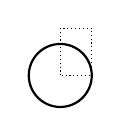
\begin{tikzpicture}
\draw[thick] (0,0) circle (.4cm);
\draw[densely dotted] (0,0) rectangle (.4cm,.6cm);
\end{tikzpicture}
\quad$\swap$\quad

\begin{tikzpicture}
\draw[thick] (0,0) circle (.4cm);
\draw[thick,fill=white] (0,0) rectangle (.6cm,.4cm);
\end{tikzpicture}\\


\null\hfill

\begin{tikzpicture}[baseline,yshift=.1cm]
\draw[thick] (0,0) circle (.4cm);
\end{tikzpicture}\quad subjective state
\hfill
$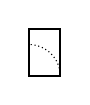
\begin{tikzpicture}[baseline,yshift=-.25cm]
\draw[thick] (0,0) rectangle (.4cm,.6cm);
\draw[densely dotted] (.4cm,0) arc (0:90:.4cm);
\end{tikzpicture}|= P$
\hfill
$
\begin{tikzpicture}[baseline]
\draw[thick,yshift=-.1cm] (0,0) rectangle (.6cm,.4cm);
\end{tikzpicture}|= Q$
\hfill\null

\vspace{5pt}\hrule\vspace{5pt}



The thread does not have the capability to do action
$\token a_x$. However, the environment might. 


The subjective view describes the thread's partial
knowledge about the shared state. The environment can have both some
of the knowledge  that the  thread has and some additional knowledge,
as long as the view of the thread and the environment are compatible. 



When that is the case, the piece
of the state corresponding to the overlap between the state and the
precondition of the action is removed, and the entire postcondition of
the action is added in its place, as shown in fig~??. 


\pgcomment{Next bit fine, maybe a bit hurried, keep simple. }


The proof of the specification of the thread $\mathbb{P}_y$ is 
now relatively straightforward. By inspection, the invariant of the while loop is stable
with respect to $I_y$. The final postcondition of $\mathbb{P}_y$ follows from the
invariant and the boolean expression of the while. We join up the
postconditions of the threads using the merge principle. Since $|/$
distributes over $**$, the subjective view simplifies to $
\shared{x|->10 * y|->10 * z|->10}{I_x\cup I_y\cup I_z} $.
Finally, we have 
\[
I_x\cup I_y\cup I_z\weakenIb{x|->10 * y|->10 * z|->10} I
\]
so, by the shift principle, we get the postcondition of $\mathbb{INC}$. 


\pgcomment{needs an ending. \colosl is brilliant, yeah.} 

\pgcomment{might include somewhere here, needn't}


Subjectivity also enables the analysis of
portions of code without access to the whole program, and allows one
to reuse the established specifications in any environment that
doesn’t violate their subjective views.


This finishes the justification of all uses of \eqref{eq:shift} in the
derivations of \S\ref{subsec:threads}, and thus the derivations
themselves.  In this section, we have informally justified
manipulations of the interference relation by semantic
arguments. However, \S\ref{sec:shiftax} will show how the reasoning
involved can be reduced to simple logical implications between
separation logic formulas that do not mention the shared state.

%% In the case of the less local predicate $G$, whenever the
%% pre-condition of the action associated with $\token a_z$ is satisfied
%% (third disjunct), it is also the case that $\cell{x}{v+1}$. In other
%% words, in all the cases where the shared state satisfies
%% $\cell{y}{v+1} * \cell{z}{v}$, it also satisfies $\cell{x}{v+1} *
%% \cell{y}{v+1} * \cell{z}{v}$. However, this information is not
%% reflected in $I$ and as a result when weakening $G$, we need to
%% stabilise the resultant assertion which proves to be very weak. To
%% remedy this, in \colosl we introduce the notion of action
%% \emph{shifting} (rewriting) with respect to the \emph{invariant} of
%% the shared state. Given $\shared{P}{I'}$, we write $\fence{} \fences
%% (P, I')$ - read ``$\fence{}$ fences $P$ with respect to $I'$'' - to
%% indicate that i) $\fence{}$ contains all states associated with $P$
%% and ii) it is closed under $I'$; that is, given any action in $I'$
%% whose pre-condition is satisfied by a state in $\fence{}$, the state
%% resulting from the action is also in $\fence{}$. For instance, given
%% the $G$ predicate of \fig\ref{fig:concurrentIncCoLoSLSpec}, we have
%% $\fence{G} \fences (P_G, I)$ where $P_G$ denotes the assertion inside
%% the box and $\fence{G}$ is as specified below.
%% \[
%% 	\begin{array}{l l}
%% 		\fence{G} = \hspace*{-5pt}& \left\{\cell{x}{v} * \cell{y}{v} * \cell{z}{v} ||| v \in \{0, \cdots 10\} \right\} \\
%% 		& \cup \left\{\cell{x}{v+1} * \cell{y}{v} * \cell{z}{v} ||| v \in \{0, \cdots 9 \} \right\} \\
%% 		& \cup \left\{\cell{x}{v+1} * \cell{y}{v+1} * \cell{z}{v} ||| v \in \{0, \cdots 9\} \right\}\\
%% 	\end{array}
%% \]
%% %as well as the action associated with its update
%% Given the above invariant, we can now \emph{shift} the action associated with $\token a_z$ in $I$ and arrive at $I'$ where
%% \[
%% 	I' \eqdef \left\{
%% 		\begin{array}{@{}l@{}}
%% 			\token a_x:\, \exsts{v} \cell{x}{v} * \cell{z}{v}  \swap  \cell{x}{v+1} * \cell{z}{v}\\
%% 			\token a_y:\, \exsts{v} \cell{x}{v+1} * \cell{y}{v}  \swap  \cell{x}{v+1} * \cell{y}{v+1}\\
%% 			\token a_z:\, \exsts{v} \cell{x}{v+1} *
%%                         \cell{y}{v+1} * \cell{z}{v} \swap\null\\
%% 			\hspace*{2cm} \cell{x}{v+1} * \cell{y}{v+1} * \cell{z}{v+1}\\
%% 		\end{array}			
%% 	\right.
%% \]
%% Note that in doing so we have neither restricted nor relaxed the action of $\token a_z$ in that it can be carried out in exactly the same states given the invariant $\fence{G}$. This is formalised by the \textsc{(Shift)} rule where $I \weakenI{\fence{}} I'$ denotes the shifting of $I$ with respect to $\fence{}$ and we defer its formalisation to \S\ref{sec:logic}.
%% \[
%% 	\text{if}\hspace*{0.25cm} \fence{} \fences (P, I) 
%% 	\hspace*{0.25cm}\text{and}\hspace*{0.25cm} I \weakenI{\fence{}} I'
%% 	\hspace*{0.25cm}\text{then}\hspace*{0.25cm}
%% 	\shared{P}{I} ===> \shared{P}{I'} \hspace*{0.5cm} \textsc{(Shift)}
%% \]
%% Given predicate $G$ of \fig\ref{fig:concurrentIncCoLoSLSpec}, we can first shift $I$ into $I'$ (specified above) using the \textsc{Shift} rule and then apply the \textsc{Forget} rule to forget variable $y$ and obtain $\shared{a_x}{I'}$.
%% %%
%% %\[
%% %	X' \eqdef \shared{\exsts{v} \cell{x}{v} * \cell{z}{v} \lor \cell{x}{v+1} * \cell{z}{v}}{I'} 
%% %\]
%% %%
%% We have almost arrived at a local specification for $\mathbb{P}_x$. However, the action of $\token a_y$ is still visible in $I'$ even though it does not affect the values of $x$ or $z$. Through interference shifting, we can not only rewrite actions with respect to the invariant, we can also \emph{forget} actions that affect \emph{none} of the states contained in the invariant. For instance, let $\fence{x} = \left\{\cell{x}{v} * \cell{z}{v} ||| v \in \{0, \cdots 10\} \right\} \cup \left\{\cell{x}{v+1} * \cell{z}{v} ||| v \in \{0, \cdots 9 \} \right\}$, then we have $\fence{X} \fences (X, I')$. In the case of the action of $\token a_y$, given any state $p$ in the action pre-condition (e.g. $p = \cell{x}{1} * \cell{y}{0}$), for an arbitrary state $s \in \fence{X}$ (e.g. $s = \cell{x}{1} * \cell{z}{0}$), \emph{all overlaps} of $p$ and $s$ ($p \meetL s = \{\cell{x}{1}\}$) are preserved by the action. We give the formal definition of overlap operator $\meetL$ in \S\ref{sec:logic}. 

%% Given $I'$ and $\fence{X}$ we can again apply the \textsc{Shift} rule in order to forget about the action of $\token a_y$ and obtain $I_x$ as specified in \fig\ref{fig:concurrentIncSubjectiveSpec}. We can take analogous steps in order to obtain subjective views $S_y$ and $S_z$ for threads $\tau_y$ and $\tau_z$. We then pass the $\token a_x$, $\token a_y$ and $\token a_z$ capabilities to $\tau_x$, $\tau_y$ and $\tau_z$ and verify $\mathbb{INC}$ as follows:
%% \[
%% \hspace*{-0.2cm}
%% \begin{array}{c}
%% 	\color{blue}{\left\{\token a_x * \token a_y *  \token a_z *  S_x * S_y * S_z \right\}}\vspace*{2pt}\\
	
%% 	\begin{array}{c || c || c}
%% 		\color{blue}{\left\{\token a_x * S_x \right\}} & \color{blue}{\left\{\token a_y * S_y \right\}} & \color{blue}{\left\{\token a_z * S_z \right\}}\\
%% 		&&\vspace*{-7pt}\\
%% 		\mathbb{P}_x & \mathbb{P}_y & \mathbb{P}_z\\
%% 		&&\vspace*{-5pt}\\

%% 		\color{blue}{
%% 			\left\{
%% 					\token a_x * S'_x
%% 			\right\}
%% 		} 
%% 		& 
%% 		\color{blue}{
%% 			\left\{
%% 				\token a_y * S'_y
%% 			\right\}
%% 		} 

%% 		&
		
%% 		\color{blue}{
%% 			\left\{
%% 				\token a_z * S'_z
%% 			\right\}
%% 		} 		
%% 		\vspace*{3pt}
%% 	\end{array}\\
%% 	\color{blue}{\left\{\token a_x * \token a_y *  \token a_z *  S'_x * S'_y * S'_z \right\}}\\
%% \end{array}
%% \]
%% with
%% \[
%% \begin{array}{l l}
%% 	S'_x \eqdef & \shared{\cell{x}{10} * \cell{z}{10} \lor \cell{x}{10} * \cell{z}{9} }{I_x}\\
%% 	S'_y \eqdef & \shared{\cell{x}{11} * \cell{y}{10} \lor \cell{x}{10} * \cell{y}{10} }{I_y}\\
%% 	S'_z \eqdef & \shared{\cell{y}{11} * \cell{z}{10} \lor \cell{y}{10} * \cell{z}{10} }{I_z}
%% \end{array}
%% \]



\pgcomment{Next bits may be usedul somewhere else, }


\pgcomment{Following too suble for section 2, should go somewhere in
  section 3.}

In particular,
an action whose precondition is satisfiable is always enabled from the
empty subjective assertion (which by definition is compatible with all
other states). 

%%%%%%%%%%%%%%%%%%%%%%%%%%%%%%%%%%
\subsection{Thread-local proofs}
\label{subsec:threads}

\pgcomment{Don't mention atomic rule until  section 3}



The proofs that $\mathbb P_x$, $\mathbb P_y$, and $\mathbb P_z$
satisfy the assertions at each program point as shown in
\fig\ref{fig:concurrentInc} are straightforward using standard
techniques from concurrency reasoning. In particular, commands in
angle brackets represent \emph{atomic sections}. Since all such
sections are operationally mutually exclusive, the program may safely
manipulate contents of the subjective region when executing an atomic
command. Logically, this translates into the following proof rule,
borrowed from concurrent abstract predicates~\cite{cap-ecoop10} (CAP):
\[
\infrule{Atomic}
        {\hoare p {\mathbb P} q\\
          \repartitions{P}{Q}{p}{q}}
        {\hoare P {<<\mathbb P>>} Q}
        {}
\]
\julescomment{TODO: explain rule}

\pgcomment{Disjoint concurrentcy rule in introduction. }

The three thread-local proofs are tied together in the main program
$\mathbb{INC}$ using two applications of the following concurrency
rule, as is standard in the concurrent separation logic family:
\[
\infrule{Parallel}
        {\hoare{P_1}{\mathbb{P}_1}{Q_1}\\
          \hoare{P_2}{\mathbb{P}_2}{Q_2}}
        {\hoare{P_1 * P_2}{\mathbb{P}_1 || \mathbb{P}_2}{Q_1 * Q_2}}
        {}
\]
More precisely, we will use the derivation below, starting from the
program state before the parallel composition and ending in the
$*$-conjunction of the preconditions of the thread threads, as
mandated by the \infrulestyle{Parallel} rule.

\pgcomment{Extension principle explained first in introduction then
  more in section 3, you judge what goes where.}



The existential quantification of capabilities is to ensure the
\emph{freshness} of the generated capabilities. The side condition $P
\containI I$ ensures that the mutations performed by actions in $I$
are confined to $P$, hence do not contradict existing views of the
shared state. This notion will be formalised in
\S\ref{subsec:extension}.



\pgcomment{KEy point of intro}

A central property of
\colosl proofs is that multiple threads can view differen,t
potentially overlapping parts of the shared state. As such, the
separating conjunction $*$ behaves as \emph{overlapping conjunction}
$\sepish$~\cite{rey-slnotes,ramification} (sometimes called
\emph{sepish}~\cite{gareth-js12}) over subjective states (in contrast
with most existing formalisms, which would use \emph{classical
  conjunction} instead).
\begin{align*}
  \shared{P}{I} &=> \shared{P}{I} * \shared{P}{I}
  \tag{\textsc{Split}}\label{eq:split}\\
  \shared{P}{I_1} * \shared{Q}{I_2} &=> \shared{P \sepish Q}{I_1\cup I_2} \tag{\textsc{Merge}}\label{eq:merge}
\end{align*}
On local states, $*$ behaves as \emph{disjoint union}, as is standard.

\julescomment{This is actually two rules! Fix the words.}

\pgcomment{ ISn't it
  double-arrow on Merge, perhaps called spilt/merge} 

This directly justifies the \eqref{eq:split} and \eqref{eq:merge}
steps of the two derivations above.

